% =====================================================================
% Use case analysis for Breakly
% Diagrams are stored in graphics/usecase/*.png
% =====================================================================

% Use case specification table: \begin{ucspec}{caption}{label} ... \end{ucspec}
\newenvironment{ucspec}[2]{%
  \begingroup
  \small
  \renewcommand{\arraystretch}{1.3}%
  \begin{longtable}{|>{\raggedright\arraybackslash}p{0.21\textwidth}|>{\raggedright\arraybackslash}p{0.71\textwidth}|}
  \caption{#1}\label{#2}\\ \hline
  \textbf{Field} & \textbf{Description} \\ \hline
  \endfirsthead
  \multicolumn{2}{c}{{\bfseries \tablename\ \thetable{} -- continued from previous page}} \\ \hline
  \textbf{Field} & \textbf{Description} \\ \hline
  \endhead
}{%
  \end{longtable}
  \endgroup
}
% One row of a specification table
\newcommand{\ucrow}[2]{\textbf{#1} & #2 \\ \hline}

The use case model of Breakly formalises the operational interactions between
the user, the system, and external supporting services during a time-boxed break.
To maintain strict consistency with the requirement baseline established in
Chapter~\ref{chap:introduction-requirements} (specifically
Section~\ref{sec:system-boundary} and Table~\ref{tab:functional-requirements}),
the model is organised into the exact same seven functional modules:
\begin{enumerate}[leftmargin=2.0em,itemsep=1pt,topsep=2pt]
  \item \textbf{Module 1 --- Authentication \& Account Management}
  \item \textbf{Module 2 --- Session Management}
  \item \textbf{Module 3 --- Space and Themes}
  \item \textbf{Module 4 --- Music (Radio)}
  \item \textbf{Module 5 --- News}
  \item \textbf{Module 6 --- Short Videos (TV)}
  \item \textbf{Module 7 --- Progress, Settings and Reliability}
\end{enumerate}

\paragraph{System Boundary and Actors.}
As identified in Section~\ref{sec:system-boundary}, the Breakly application
interacts with one primary human actor and three external supporting actors:
\begin{itemize}[leftmargin=1.8em,itemsep=2pt,topsep=2pt]
  \item \textbf{User} -- the primary human actor (the Breakly user) who directly
        drives application interactions to configure, initiate, and enjoy bounded
        break sessions. UC-01 and UC-02 are performed before the user is signed in;
        all other use cases require a signed-in user.
  \item \textbf{Mobile OS} -- the platform service that manages the application
        lifecycle (foreground, background, locked screen), provides the background
        audio session that maintains music playback when the device is locked,
        and provides secure hardware-backed storage for authentication tokens.
  \item \textbf{Auth \& Sync Service} -- the secure cloud backend responsible
        for account credential validation, user profile storage, and cross-device
        synchronisation of session records and streaks.
  \item \textbf{Content Providers} -- the external services delivering digital
        media feeds. In detailed subsystem models, this actor is specialized into
        three concrete content providers: the \textbf{Music Content Provider}
        (streaming audio tracks), the \textbf{News Feed Content Provider} (RSS/Atom syndication),
        and the \textbf{Video Content Provider} (curated finite short-video clips).
\end{itemize}

% ---------------------------------------------------------------------
\subsection{Overall Use Case}
\label{sec:overall-usecase}

Figure~\ref{fig:uc-overall} presents the overall use case diagram for the
Breakly application. It groups the fourteen core use cases into the seven
functional modules defined in Chapter~\ref{chap:introduction-requirements} and
illustrates the participation of both the primary actor and the secondary
supporting actors. Table~\ref{tab:usecase-list} outlines the complete use case
inventory alongside its traceability to the User Requirements (UR-01--UR-20)
and Functional Requirements (FR 1.1--FR 7.8); every requirement specified in
Chapter~\ref{chap:introduction-requirements} is completely covered.

\begin{figure}[H]
  \centering
  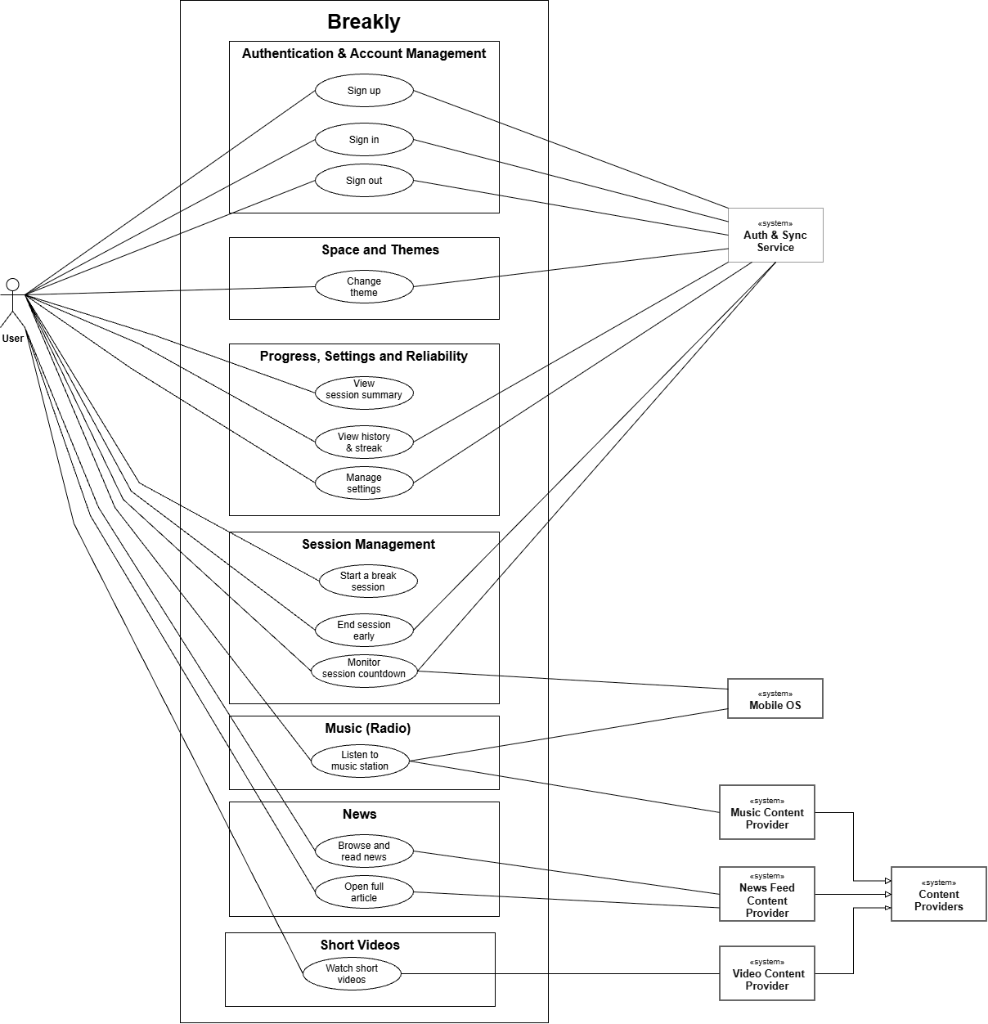
\includegraphics[width=0.92\textwidth,height=0.78\textheight,keepaspectratio]{graphics/usecase/uc00_overall.png}
  \caption{Overall use case diagram of Breakly}
  \label{fig:uc-overall}
\end{figure}

\clearpage

\begingroup
\small
\renewcommand{\arraystretch}{1.25}
\begin{longtable}{|>{\centering\arraybackslash}p{1.3cm}|>{\raggedright\arraybackslash}p{3.5cm}|>{\raggedright\arraybackslash}p{4.5cm}|>{\raggedright\arraybackslash}p{2.9cm}|>{\centering\arraybackslash}p{1.6cm}|}
\caption{Use case list and traceability to functional requirements}
\label{tab:usecase-list}\\ \hline
\textbf{ID} & \textbf{Use Case} & \textbf{Module} & \textbf{Related FR (UR)} & \textbf{Priority} \\ \hline
\endfirsthead
\multicolumn{5}{c}{{\bfseries \tablename\ \thetable{} -- continued from previous page}} \\ \hline
\textbf{ID} & \textbf{Use Case} & \textbf{Module} & \textbf{Related FR (UR)} & \textbf{Priority} \\ \hline
\endhead
UC-01 & Sign up & Module 1 --- Authentication \& Account Management & FR 1.1 (UR-01) & Must \\ \hline
UC-02 & Sign in & Module 1 --- Authentication \& Account Management & FR 1.2 (UR-01) & Must \\ \hline
UC-03 & Sign out & Module 1 --- Authentication \& Account Management & FR 1.3 (UR-01) & Must \\ \hline
UC-04 & Start a break session & Module 2 --- Session Management & FR 2.1, 2.2, 2.3, 3.1\newline(UR-02, 03, 04, 07) & Must \\ \hline
UC-05 & Monitor session countdown & Module 2 --- Session Management & FR 2.3, 2.4, 2.5, 2.6, 7.2\newline(UR-04, 05, 18) & Must \\ \hline
UC-06 & End session early & Module 2 --- Session Management & FR 2.7 (UR-06) & Should \\ \hline
UC-07 & Change theme & Module 3 --- Space and Themes & FR 3.1, 3.2, 3.3\newline(UR-07, 08) & Must \\ \hline
UC-08 & Listen to music station & Module 4 --- Music (Radio) & FR 4.1--4.5, 7.7, 7.8\newline(UR-09, 10, 20) & Must \\ \hline
UC-09 & Browse and read news & Module 5 --- News & FR 5.1--5.4, 7.7, 7.8\newline(UR-11, 12, 20) & Must \\ \hline
UC-10 & Open full article & Module 5 --- News & FR 5.5 (UR-13) & Should \\ \hline
UC-11 & Watch short videos & Module 6 --- Short Videos (TV) & FR 6.1--6.3, 4.5, 7.7, 7.8\newline(UR-14, 15, 20) & Should \\ \hline
UC-12 & View session summary & Module 7 --- Progress, Settings and Reliability & FR 7.1 (UR-16) & Should \\ \hline
UC-13 & View history and streak & Module 7 --- Progress, Settings and Reliability & FR 7.2, 7.3, 7.4, 7.8\newline(UR-17, 18, 20) & Must \\ \hline
UC-14 & Manage settings & Module 7 --- Progress, Settings and Reliability & FR 7.5, 7.6 (UR-19) & Should \\ \hline
\end{longtable}
\endgroup

% ---------------------------------------------------------------------
\subsection{Detailed Use Case Diagrams}
\label{sec:detailed-usecase}

The following diagrams provide refined specifications for each functional
module. Solid association lines connect actors to the use cases they participate
in. Dashed dependency arrows labelled \textit{\guillemotleft include\guillemotright}
indicate mandatory behaviour executed as an inherent part of the base use case,
while dashed arrows labelled \textit{\guillemotleft extend\guillemotright}
represent optional or conditional behaviour that augments the base workflow.

\paragraph{Module 1 --- Authentication \& Account Management.}
Figure~\ref{fig:uc-account} details the account lifecycle workflows. A user
who is not yet signed in initiates Sign up (UC-01) or Sign in (UC-02), both of which
validate credentials against the Auth \& Sync Service. Upon successful authentication,
an access token is stored in secure device storage (NFR-04), enabling persistent
sessions across app restarts. Sign out (UC-03) safely revokes the token, clears
stored tokens from secure storage, and purges cached session history from the device.

\begin{figure}[H]
  \centering
  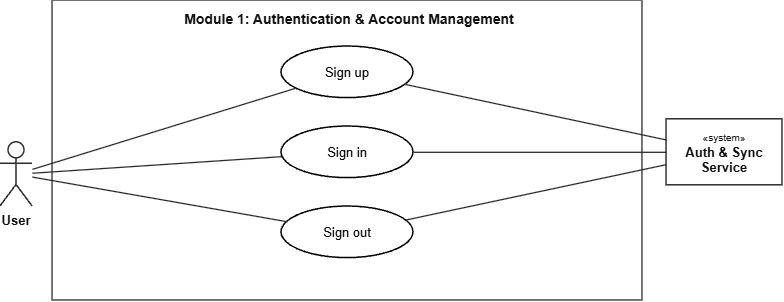
\includegraphics[width=0.95\textwidth,height=0.45\textheight,keepaspectratio]{graphics/usecase/uc01_account.png}
  \caption{Use case diagram for Module 1 --- Authentication \& Account Management}
  \label{fig:uc-account}
\end{figure}

\paragraph{Module 2 --- Session Management.}
Figure~\ref{fig:uc-session} specifies the core break-session lifecycle. Starting
a session (UC-04) encapsulates duration selection (10, 20, or 30 minutes, defaulting
to 20) and triggering a service via Space interactive objects. During an active
session, the countdown is calculated dynamically from the stored start and target end
timestamps, while the Mobile OS lifecycle management ensures audio continuity
across background and screen-locked states (UC-05). As the session approaches its
conclusion, the system delivers a gentle one-minute in-app reminder, and upon timer
expiration automatically halts playback and persists a completed session record.
End session early (UC-06) extends the countdown workflow to enable safe user-confirmed
termination, saving the session as ended early.

\begin{figure}[H]
  \centering
  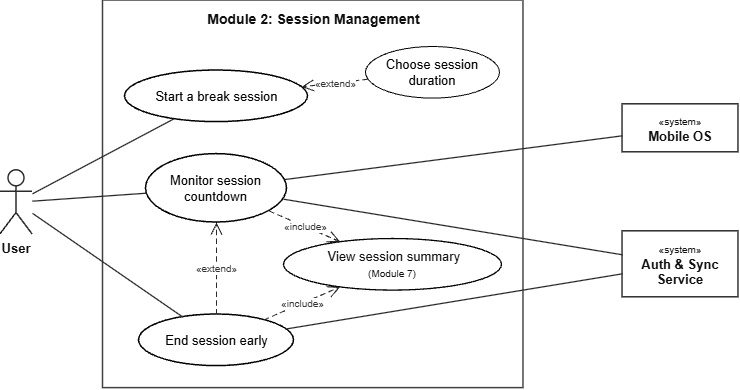
\includegraphics[width=0.95\textwidth,height=0.5\textheight,keepaspectratio]{graphics/usecase/uc02_session.png}
  \caption{Use case diagram for Module 2 --- Session Management}
  \label{fig:uc-session}
\end{figure}

\paragraph{Module 3 --- Space and Themes.}
As illustrated in Figure~\ref{fig:uc-space-theme}, the Home Space acts as the
primary visual anchor, loading the user's selected theme (Cozy Room or Garden)
from local storage with graceful fallback backgrounds in case of asset loading errors.
Changing themes (UC-07) enables previewing and persisting aesthetic selections
locally and to the cloud profile without altering the spatial positioning of interactive objects.

\begin{figure}[H]
  \centering
  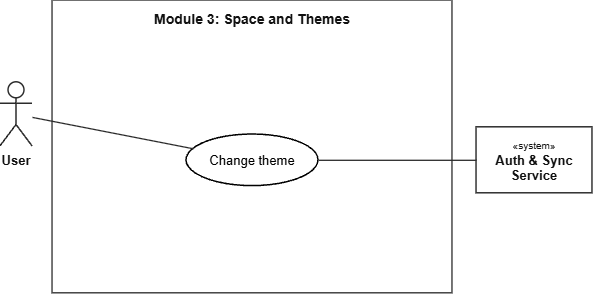
\includegraphics[width=0.85\textwidth,height=0.4\textheight,keepaspectratio]{graphics/usecase/uc03_space_theme.png}
  \caption{Use case diagram for Module 3 --- Space and Themes}
  \label{fig:uc-space-theme}
\end{figure}

\paragraph{Module 4 --- Music (Radio).}
Figure~\ref{fig:uc-music} captures the music service. The user selects a station
category (Lo-fi, Piano, Acoustic or Nature) and listens to tracks from the Music
Content Provider (UC-08); playback continues across screens and on the locked
screen through the Mobile OS audio session, and pauses automatically while the
TV is open. While music is playing, the user may control playback on the Radio
screen (play/pause, next track, volume) or from the mini-player on the News and
Article screens; both extend UC-08.

\begin{figure}[H]
  \centering
  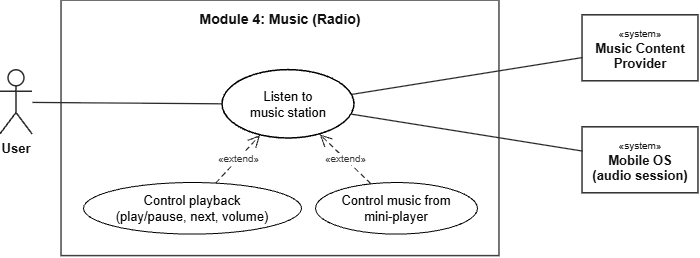
\includegraphics[width=0.95\textwidth,height=0.45\textheight,keepaspectratio]{graphics/usecase/uc04_music.png}
  \caption{Use case diagram for Module 4 --- Music (Radio)}
  \label{fig:uc-music}
\end{figure}

\paragraph{Module 5 --- News.}
Figure~\ref{fig:uc-news} outlines the news reading experience. Browsing news
(UC-09) loads curated feeds from the News Feed Content Provider and supports direct
in-app reading with full countdown visibility. Category filtering and pull-to-refresh
actions enhance feed navigation, while opening the complete source article
in an in-app browser view (UC-10) extends the reading workflow.

\begin{figure}[H]
  \centering
  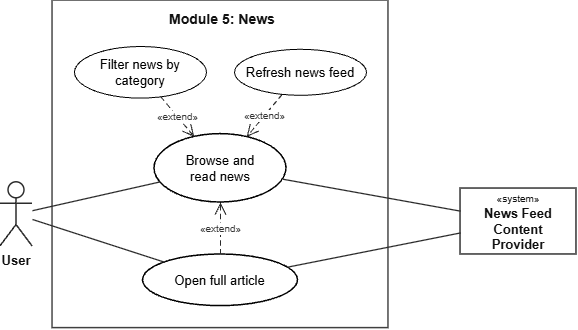
\includegraphics[width=0.95\textwidth,height=0.45\textheight,keepaspectratio]{graphics/usecase/uc05_news.png}
  \caption{Use case diagram for Module 5 --- News}
  \label{fig:uc-news}
\end{figure}

\paragraph{Module 6 --- Short Videos (TV).}
Figure~\ref{fig:uc-videos} models the finite video feed in Module 6 --- Short
Videos (TV), which deliberately breaks away from infinite algorithmic doomscrolling.
Watching short videos (UC-11) retrieves a bounded feed of at most ten clips navigated
via vertical swiping, and invariably terminates with an explicit end card.
Control video playback extends the viewing workflow to allow toggling playback
and audio muting at any step, and the user can seamlessly return to the Home Space
upon reaching the end card.

\begin{figure}[H]
  \centering
  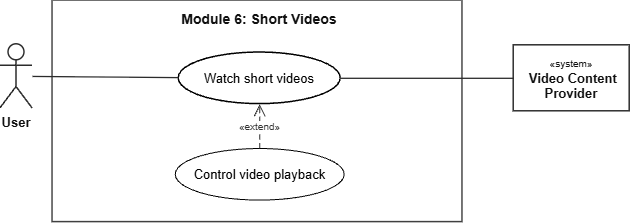
\includegraphics[width=0.9\textwidth,height=0.42\textheight,keepaspectratio]{graphics/usecase/uc06_videos.png}
  \caption{Use case diagram for Module 6 --- Short Videos (TV)}
  \label{fig:uc-videos}
\end{figure}

\paragraph{Module 7 --- Progress, Settings and Reliability.}
Figure~\ref{fig:uc-progress} unifies progress tracking, administrative,
and resilience use cases in Module 7 --- Progress, Settings and Reliability.
At session conclusion (via UC-05 or UC-06), the session record is persisted and
synchronised; viewing the session summary (UC-12) calculates and presents engagement
metrics. Viewing history and streak (UC-13) tracks habit consistency, retrieving
locally cached records when offline. In Settings (UC-14), the user turns the
gentle one-minute reminder on or off, and viewing the content credits extends
this use case.

\begin{figure}[H]
  \centering
  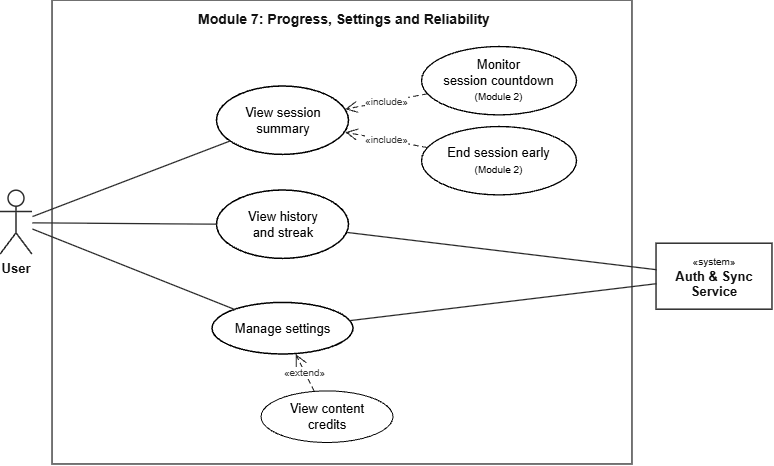
\includegraphics[width=0.95\textwidth,height=0.45\textheight,keepaspectratio]{graphics/usecase/uc07_progress_settings.png}
  \caption{Use case diagram for Module 7 --- Progress, Settings and Reliability}
  \label{fig:uc-progress}
\end{figure}

% ---------------------------------------------------------------------
\subsection{Use Case Descriptions}
\label{sec:usecase-descriptions}

This subsection specifies the fourteen use cases listed in
Table~\ref{tab:usecase-list}. Each specification states the actors, the
related functional requirements, the preconditions and trigger, the normal
flow, the alternative flows (other valid ways to reach the goal), the exception
flows (errors and failures), and the postconditions. The specifications are the
basis for the sequence diagrams in Chapter~\ref{chap:design} and for the test
cases in Chapter~\ref{chap:implementation-testing}.

% ---------------------------- UC-01 ----------------------------------
\begin{ucspec}{UC-01: Sign up}{tab:uc-01}
\ucrow{Use Case ID}{UC-01}
\ucrow{Module}{Module 1 --- Authentication \& Account Management}
\ucrow{Primary Actor}{User}
\ucrow{Secondary Actor}{Auth \& Sync Service}
\ucrow{Description}{A new user creates a Breakly account with an email address and a password so that sessions and streaks can be saved.}
\ucrow{Related FR}{FR 1.1 (UR-01)}
\ucrow{Priority}{Must}
\ucrow{Preconditions}{The app is installed and opened. The user is not signed in.}
\ucrow{Trigger}{The user selects \textit{Create account} on the Sign In screen.}
\ucrow{Normal Flow}{%
1. The system displays the sign-up form with email and password fields.\newline
2. The user enters an unused email address and a password of at least 8 characters.\newline
3. The user submits the form.\newline
4. The system validates that the email format is valid and the password has at least 8 characters.\newline
5. The system sends the registration request to the Auth \& Sync Service.\newline
6. The Auth \& Sync Service creates the account and returns an access token.\newline
7. The system stores the access token securely in device storage (NFR-04) and displays the Home Space with the default Cozy Room theme.}
\ucrow{Alternative Flows}{%
A1. The user already has an account: at step 2 the user selects \textit{Sign in} and continues with UC-02.}
\ucrow{Exception Flows}{%
E1. Invalid email format or password shorter than 8 characters: at step 4 the system shows an inline error next to the field and does not submit the form.\newline
E2. Email already registered: at step 6 the service rejects the request; the system shows an error message and no second account is created.\newline
E3. No connection or service unavailable: the system shows an offline message with a \textit{Retry} option; no account is created.}
\ucrow{Postconditions}{%
Success: a new account exists, the access token is stored in secure device storage, and the user is authenticated on the Home Space.\newline
Failure: no account is created and the user stays on the sign-up form.}
\end{ucspec}

% ---------------------------- UC-02 ----------------------------------
\begin{ucspec}{UC-02: Sign in}{tab:uc-02}
\ucrow{Use Case ID}{UC-02}
\ucrow{Module}{Module 1 --- Authentication \& Account Management}
\ucrow{Primary Actor}{User}
\ucrow{Secondary Actor}{Auth \& Sync Service}
\ucrow{Description}{A registered user signs in with email and password and remains signed in until signing out.}
\ucrow{Related FR}{FR 1.2 (UR-01)}
\ucrow{Priority}{Must}
\ucrow{Preconditions}{The user has an existing account and is not signed in on this device.}
\ucrow{Trigger}{The user opens the app without a saved sign-in, or selects \textit{Sign in}.}
\ucrow{Normal Flow}{%
1. The system displays the sign-in form.\newline
2. The user enters the registered email and password.\newline
3. The user submits the form.\newline
4. The system validates that both fields are non-empty and sends the credentials to the Auth \& Sync Service.\newline
5. The service validates credentials and returns an access token.\newline
6. The system stores the access token in secure device storage (NFR-04).\newline
7. The system displays the Home Space with the user's saved theme.}
\ucrow{Alternative Flows}{%
A1. Saved token at launch: when the app is reopened and a valid access token is found in secure device storage, the system skips steps 1--6 and navigates directly to the Home Space.\newline
A2. Launch while offline with saved token: if the device is offline upon launch but contains a valid stored access token, the system validates the local token and shows the Home Space with cached data.\newline
A3. The user has no account: the user selects \textit{Create account} and continues with UC-01.}
\ucrow{Exception Flows}{%
E1. Empty field: at step 4 the system highlights the missing field and does not submit.\newline
E2. Incorrect credentials: at step 5 the service rejects the request; the system shows an error message and the user stays on the Sign In screen.\newline
E3. No connection or service unavailable: the system shows an offline message with a \textit{Retry} option.\newline
E4. Expired or revoked token: if a stored token is rejected by the server, the system purges the invalid token from secure storage, displays an expiration alert, and routes to the Sign In screen.}
\ucrow{Postconditions}{%
Success: the user is signed in, the access token is stored in secure storage, and the session persists across app restarts.\newline
Failure: the user remains signed out.}
\end{ucspec}

% ---------------------------- UC-03 ----------------------------------
\begin{ucspec}{UC-03: Sign out}{tab:uc-03}
\ucrow{Use Case ID}{UC-03}
\ucrow{Module}{Module 1 --- Authentication \& Account Management}
\ucrow{Primary Actor}{User}
\ucrow{Secondary Actor}{Auth \& Sync Service}
\ucrow{Description}{A signed-in user signs out so that the account and its history are no longer accessible on the device.}
\ucrow{Related FR}{FR 1.3 (UR-01)}
\ucrow{Priority}{Must}
\ucrow{Preconditions}{The user is signed in.}
\ucrow{Trigger}{The user selects \textit{Sign out} on the Settings screen.}
\ucrow{Normal Flow}{%
1. The user selects \textit{Sign out}.\newline
2. The system revokes the session on the Auth \& Sync Service.\newline
3. The system removes the stored access token from secure device storage.\newline
4. The system clears the previous account's session history and cached data from active memory and UI views.\newline
5. The system displays the Sign In screen.}
\ucrow{Alternative Flows}{%
A1. Unsynced session records exist: before step 3, if pending records exist in the local queue, the system attempts an immediate cloud upload before signing out.\newline
A2. A break session is active: before step 2 the system asks the user to confirm ending the session. If the user confirms, the session is stopped and saved with status \textit{ended\_early}, and sign-out continues at step 2. If the user cancels, sign-out is aborted and the session continues.}
\ucrow{Exception Flows}{%
E1. Offline sign-out: if network connectivity is unavailable at step 2, the system warns the user that pending records will remain queued locally under the user's account ID, removes the access token from secure storage, and displays the Sign In screen; device sign-out is never blocked by network failure.}
\ucrow{Postconditions}{%
The access token is removed from secure device storage, active session data is purged from memory, the Sign In screen is shown, and the previous account's session history is no longer accessible on the device.}
\end{ucspec}

% ---------------------------- UC-04 ----------------------------------
\begin{ucspec}{UC-04: Start a break session}{tab:uc-04}
\ucrow{Use Case ID}{UC-04}
\ucrow{Module}{Module 2 --- Session Management}
\ucrow{Primary Actor}{User}
\ucrow{Secondary Actor}{--}
\ucrow{Description}{The user taps the radio, the newspaper or the TV in the Space to start a time-boxed session with the selected duration and open the matching service.}
\ucrow{Related FR}{FR 2.1, FR 2.2, FR 2.3, FR 3.1 (UR-02, UR-03, UR-04, UR-07)}
\ucrow{Priority}{Must}
\ucrow{Preconditions}{The user is signed in, the Home Space is displayed, and no session is active.}
\ucrow{Trigger}{The user views the Home Space with no active session.}
\ucrow{Normal Flow}{%
1. The system displays the Home Space scene with the labelled interactive objects -- radio (Music), newspaper (News) and TV (Short Videos), each with a touch target of at least 48~dp -- and the duration selector with 20 minutes selected by default.\newline
2. The user taps an object (a session can be started in at most two taps from the Home Space).\newline
3. The system creates an active session with status \textit{in\_progress}, records the start timestamp and the target end timestamp, and starts the countdown.\newline
4. The system locks the duration selector while the session is active.\newline
5. The system opens the matching service: Radio (UC-08), News (UC-09) or TV (UC-11).\newline
6. The system shows the remaining time on every screen and updates it every second (UC-05).}
\ucrow{Alternative Flows}{%
A1. Choose session duration: at step 1 the user selects 10, 20 or 30 minutes; exactly one option is selected at a time, and the flow returns to step 1 with the new duration selected.}
\ucrow{Exception Flows}{%
E1. Content fails to load upon opening service: the system shows a loading indicator followed by an offline or error message with a \textit{Retry} option; the countdown keeps running.}
\ucrow{Postconditions}{%
A session is active with a stored start time and duration, the countdown is visible, and the selected service is open.}
\end{ucspec}

% ---------------------------- UC-05 ----------------------------------
\begin{ucspec}{UC-05: Monitor session countdown}{tab:uc-05}
\ucrow{Use Case ID}{UC-05}
\ucrow{Module}{Module 2 --- Session Management}
\ucrow{Primary Actor}{User}
\ucrow{Secondary Actor}{Mobile OS; Auth \& Sync Service}
\ucrow{Description}{While a session is active, the system tracks remaining time across screens and in background states, provides a gentle in-app one-minute notice, halts playback upon expiration, and persists a completed session record.}
\ucrow{Related FR}{FR 2.3, FR 2.4, FR 2.5, FR 2.6, FR 7.2 (UR-04, UR-05, UR-18)}
\ucrow{Priority}{Must}
\ucrow{Preconditions}{A session has been started (UC-04).}
\ucrow{Trigger}{The countdown starts; the use case continues until the remaining time reaches zero.}
\ucrow{Normal Flow}{%
1. The system displays the remaining countdown in minutes and seconds ($mm:ss$) on the Home Space, Radio, News, Article, and TV screens, recalculating remaining time each second from the target end timestamp.\newline
2. The user consumes content; the application may transition to the background or the device screen may be locked.\newline
3. The system maintains countdown accuracy against real time upon return (NFR-02: remaining time is 7 minutes $\pm 2$ seconds after 3 minutes in background during a 10-minute session).\newline
4. When 60 seconds remain and the application is in the foreground, the system displays a non-blocking in-app ``One minute left'' message for at least 3 seconds and highlights the timer visually.\newline
5. When the countdown reaches zero ($00:00$), the system automatically stops music and video playback immediately (even when backgrounded or locked, managed through the Mobile OS audio session).\newline
6. The system marks the session record as \textit{completed}, packages the start time, duration, and services used, and persists it to local storage and the Auth \& Sync Service.\newline
7. Include View session summary (UC-12).}
\ucrow{Alternative Flows}{%
A1. One-minute notice disabled in Settings: step 4 shows no message.\newline
A2. App backgrounded or screen locked at the 60-second mark: the in-app gentle notice is omitted (silent) to avoid unsolicited system push notifications (NFR-05).\newline
A3. Time runs out while backgrounded or locked: audio playback terminates immediately; upon reopening the app, the system detects the completed session and displays the Session Summary screen (UC-12).\newline
A4. End session early: at any time between step 1 and step 5 the user selects \textit{End session}; the flow continues in UC-06 and this use case ends.}
\ucrow{Exception Flows}{%
E1. Offline at session completion: the completed record is stored in the local SQLite queue and uploaded automatically when connectivity returns.}
\ucrow{Postconditions}{%
The session has ended, playback has stopped, and the session record (marked \textit{completed}) is saved on the device and, when online, on the Auth \& Sync Service.}
\end{ucspec}

% ---------------------------- UC-06 ----------------------------------
\begin{ucspec}{UC-06: End session early}{tab:uc-06}
\ucrow{Use Case ID}{UC-06}
\ucrow{Module}{Module 2 --- Session Management}
\ucrow{Primary Actor}{User}
\ucrow{Secondary Actor}{Auth \& Sync Service}
\ucrow{Description}{The user stops an active session before the countdown reaches zero, after confirming the action.}
\ucrow{Related FR}{FR 2.7 (UR-06)}
\ucrow{Priority}{Should}
\ucrow{Preconditions}{A session is active.}
\ucrow{Trigger}{The user selects \textit{End session}.}
\ucrow{Normal Flow}{%
1. The user selects \textit{End session}.\newline
2. The system shows a confirmation dialog.\newline
3. The user confirms.\newline
4. The system immediately stops music and video playback and halts the countdown.\newline
5. The system records the session with the actual time used, marks its status as \textit{ended\_early} (which does not qualify as a completed break for streak calculation), and saves it to local storage and the Auth \& Sync Service.\newline
6. Include View session summary (UC-12).}
\ucrow{Alternative Flows}{%
A1. The user cancels at step 3: the dialog closes and the session continues unchanged.\newline
A2. The countdown reaches zero while the dialog is open: the dialog closes and the session ends automatically as in UC-05.}
\ucrow{Exception Flows}{%
E1. Offline at early termination: the record is stored locally in the queue and uploaded when the connection returns.}
\ucrow{Postconditions}{%
Confirmed: the session has ended, status is marked \textit{ended\_early}, and its record is saved.\newline
Cancelled: the session and its countdown are unchanged.}
\end{ucspec}

% ---------------------------- UC-07 ----------------------------------
\begin{ucspec}{UC-07: Change theme}{tab:uc-07}
\ucrow{Use Case ID}{UC-07}
\ucrow{Module}{Module 3 --- Space and Themes}
\ucrow{Primary Actor}{User}
\ucrow{Secondary Actor}{Auth \& Sync Service}
\ucrow{Description}{The user changes the look of the Home Space between the Cozy Room and Garden themes, and the choice is remembered.}
\ucrow{Related FR}{FR 3.1, FR 3.2, FR 3.3 (UR-07, UR-08)}
\ucrow{Priority}{Must}
\ucrow{Preconditions}{The user is signed in.}
\ucrow{Trigger}{The user opens the Theme Selector.}
\ucrow{Normal Flow}{%
1. The system lists the Cozy Room and Garden themes, each with a preview image and a name, and marks the current theme.\newline
2. The user selects a theme.\newline
3. The user applies the theme.\newline
4. The system changes the Home Space background and colours; the layout and the positions of the radio, newspaper, and TV stay the same.\newline
5. The system persists the selected theme in local storage immediately and syncs with account preferences on the Auth \& Sync Service when online.}
\ucrow{Alternative Flows}{%
A1. First launch: no theme has been saved, so the system shows Cozy Room by default.\newline
A2. The user leaves the Theme Selector without applying: the current theme is kept.\newline
A3. The user selects the theme that is already active: nothing changes.}
\ucrow{Exception Flows}{%
E1. The theme image cannot be loaded: the system shows a fallback background in the theme colours and the objects remain usable.}
\ucrow{Postconditions}{%
The selected theme is shown on the Home Space and is shown again after the app is closed and reopened.}
\end{ucspec}

% ---------------------------- UC-08 ----------------------------------
\begin{ucspec}{UC-08: Listen to music station}{tab:uc-08}
\ucrow{Use Case ID}{UC-08}
\ucrow{Module}{Module 4 --- Music (Radio)}
\ucrow{Primary Actor}{User}
\ucrow{Secondary Actor}{Music Content Provider; Mobile OS}
\ucrow{Description}{The user picks a music station category and controls playback; music keeps playing across screens and when the device is locked, and automatically pauses while the TV is open.}
\ucrow{Related FR}{FR 4.1--4.5, 7.7, 7.8 (UR-09, UR-10, UR-20)}
\ucrow{Priority}{Must}
\ucrow{Preconditions}{A session is active (started from the radio in UC-04 or already running).}
\ucrow{Trigger}{The user taps the radio in the Space, either to start a session (UC-04) or while a session is already active; in the second case the countdown continues without restarting.}
\ucrow{Normal Flow}{%
1. The system shows the Radio screen with the categories (for example Lo-fi, Piano, Acoustic and Nature).\newline
2. The user selects a category (only one category is selected at a time).\newline
3. The system loads a track from the Music Content Provider and starts playback, showing the title, artist and artwork.\newline
4. When the user moves to another screen, playback continues and a mini-player with a play/pause control is shown on the News and Article screens.\newline
5. When the user locks the device, playback continues under the Mobile OS audio session.\newline
6. When the session ends, the system stops playback automatically.}
\ucrow{Alternative Flows}{%
A1. The user selects another category: the system switches to a track from the new category.\newline
A2. The user opens the TV screen while music plays: audio playback pauses automatically, and resumes from the paused position when the user leaves the TV screen (unless the user had paused playback manually).\newline
A3. The user had paused the music manually before opening the TV: it stays paused after leaving the TV.\newline
A4. Control playback (play/pause, next, volume): at any time between step 3 and step 6 the user uses the controls on the Radio screen. Pause stops the audio and the control changes to play; play resumes from the same position; next track starts another track of the selected category; the volume control changes the playback volume. The flow returns to the step where it was interrupted.\newline
A5. Control music from mini-player: while the News or Article screen is shown (step 4), the user taps play/pause on the mini-player; playback pauses or resumes and the flow returns to step 4.}
\ucrow{Exception Flows}{%
E1. The track cannot be loaded: the system shows a loading indicator, then an error message with a \textit{Retry} option; the countdown keeps running.\newline
E2. No connection: the system shows an offline message with a \textit{Retry} option.}
\ucrow{Postconditions}{%
Playback reflects the user's last action, and total listening duration is tracked for inclusion in the session summary.}
\end{ucspec}

% ---------------------------- UC-09 ----------------------------------
\begin{ucspec}{UC-09: Browse and read news}{tab:uc-09}
\ucrow{Use Case ID}{UC-09}
\ucrow{Module}{Module 5 --- News}
\ucrow{Primary Actor}{User}
\ucrow{Secondary Actor}{News Feed Content Provider}
\ucrow{Description}{The user browses the latest articles, optionally filters or refreshes the list, and reads an article inside the app (an article is counted as opened once its detail view is displayed).}
\ucrow{Related FR}{FR 5.1--5.4, 7.7, 7.8 (UR-11, UR-12, UR-20)}
\ucrow{Priority}{Must}
\ucrow{Preconditions}{A session is active.}
\ucrow{Trigger}{The user taps the newspaper in the Space, either to start a session (UC-04) or while a session is already active.}
\ucrow{Normal Flow}{%
1. The system shows placeholder cards while it loads the configured feeds.\newline
2. The system lists the articles from newest to oldest; each card shows the title, source, publication time, and an image when available.\newline
3. The user taps an article card.\newline
4. The system opens the Article screen inside the app with the title, source, publication time, image, and content provided by the feed; the countdown stays visible.\newline
5. The user goes back to the article list.}
\ucrow{Alternative Flows}{%
A1. Filter news by category: at step 2 the user selects a category chip and only articles of that category are listed; the all-articles chip restores the full list.\newline
A2. Refresh news feed: at step 2 the user pulls the list down; the feeds are reloaded and newer articles appear at the top.\newline
A3. Open full article: at step 4 the user selects \textit{Read full article} and continues with UC-10.}
\ucrow{Exception Flows}{%
E1. No connection on first load: the system shows an offline message with a \textit{Retry} option; the countdown keeps running.\newline
E2. Refresh fails: the system shows an error message and keeps the existing list.\newline
E3. The selected category has no articles: the system shows an empty-state message.}
\ucrow{Postconditions}{%
The articles the user opened are counted for the session summary. No data on the server is modified.}
\end{ucspec}

% ---------------------------- UC-10 ----------------------------------
\begin{ucspec}{UC-10: Open full article}{tab:uc-10}
\ucrow{Use Case ID}{UC-10}
\ucrow{Module}{Module 5 --- News}
\ucrow{Primary Actor}{User}
\ucrow{Secondary Actor}{News Feed Content Provider (source website)}
\ucrow{Description}{The user opens the full article on the source website without leaving the session.}
\ucrow{Related FR}{FR 5.5 (UR-13)}
\ucrow{Priority}{Should}
\ucrow{Preconditions}{The Article screen is open (UC-09) and the article has a source link.}
\ucrow{Trigger}{The user selects \textit{Read full article}.}
\ucrow{Normal Flow}{%
1. The user selects \textit{Read full article}.\newline
2. The system opens the source page in an in-app browser view (\texttt{expo-web-browser}).\newline
3. The user reads the original web article while the native countdown continues running in the background.\newline
4. The user closes the browser view.\newline
5. The system shows the Article screen again; the countdown has kept running.}
\ucrow{Alternative Flows}{%
A1. The session ends while the browser view is open: the system automatically closes the in-app browser view and displays the Session Summary screen (UC-12).}
\ucrow{Exception Flows}{%
E1. The source page cannot be loaded or there is no connection: the browser view shows an error and the user can return to the Article screen.}
\ucrow{Postconditions}{%
The user is back on the Article screen and the session countdown is unaffected.}
\end{ucspec}

% ---------------------------- UC-11 ----------------------------------
\begin{ucspec}{UC-11: Watch short videos}{tab:uc-11}
\ucrow{Use Case ID}{UC-11}
\ucrow{Module}{Module 6 --- Short Videos (TV)}
\ucrow{Primary Actor}{User}
\ucrow{Secondary Actor}{Video Content Provider}
\ucrow{Description}{The user watches a finite feed of short videos in full screen, which ends with an end card instead of endless scrolling (a video is counted as watched once played for at least 3 seconds).}
\ucrow{Related FR}{FR 6.1--6.3, 4.5, 7.7, 7.8 (UR-14, UR-15, UR-20)}
\ucrow{Priority}{Should}
\ucrow{Preconditions}{A session is active.}
\ucrow{Trigger}{The user taps the TV in the Space, either to start a session (UC-04) or while a session is already active.}
\ucrow{Normal Flow}{%
1. The system loads a finite feed of at most 10 clips for the current break session.\newline
2. The first clip starts playing in full screen and a progress indicator shows its position in the feed.\newline
3. The user swipes up for the next clip or down for the previous clip.\newline
4. After the last clip, the system shows an end card with a closing message and plays no further clip.\newline
5. The user returns to the Home Space from the end card.}
\ucrow{Alternative Flows}{%
A1. Music is playing when the TV opens: the music pauses automatically and resumes when the user leaves the TV (UC-08).\newline
A2. Reopening the TV after reaching the end card: within the same session, reopening the TV shows the end card directly, preventing endless scrolling.\newline
A3. Early exit: the user navigates back to the Home Space before the end card; video playback stops immediately.\newline
A4. The user swipes down on the first clip: the first clip stays on screen.\newline
A5. Control video playback: at any time between step 2 and step 4 the user taps the video to toggle between pause and play, or uses the mute control to switch the sound off or on; the flow returns to the step where it was interrupted.}
\ucrow{Exception Flows}{%
E1. The feed cannot be loaded or there is no connection: the system shows an offline or error message with a \textit{Retry} option; the countdown keeps running.\newline
E2. A single clip fails to play: the system shows an error state for that clip with a \textit{Retry} option.}
\ucrow{Postconditions}{%
No more than 10 clips have been shown, video playback ceases, and the number of videos watched ($\ge 3$s) is recorded for the session summary.}
\end{ucspec}

% ---------------------------- UC-12 ----------------------------------
\begin{ucspec}{UC-12: View session summary}{tab:uc-12}
\ucrow{Use Case ID}{UC-12}
\ucrow{Module}{Module 7 --- Progress, Settings and Reliability}
\ucrow{Primary Actor}{User}
\ucrow{Secondary Actor}{--}
\ucrow{Description}{When a session ends, the user reviews a summary of break time used and content engagement metrics, and returns to the Home Space.}
\ucrow{Related FR}{FR 7.1 (UR-16)}
\ucrow{Priority}{Should}
\ucrow{Preconditions}{A session has just ended automatically (UC-05) or early (UC-06).}
\ucrow{Trigger}{The session ends.}
\ucrow{Normal Flow}{%
1. The system calculates engagement metrics from the concluded session: total duration used, music listening time, number of articles opened, and number of videos watched (clips played $\ge 3$s).\newline
2. The system displays the Session Summary screen presenting these metrics and the updated streak count.\newline
3. The user reviews the metrics and taps \textit{Done}.\newline
4. The system navigates back to the Home Space with the updated daily streak.}
\ucrow{Alternative Flows}{%
A1. The session ended while the app was in the background: the summary is shown when the app is reopened.\newline
A2. A service was not used: its value is shown as zero in the summary metrics.}
\ucrow{Exception Flows}{%
E1. Metric computation error: default fallback metrics (total duration only) are shown.}
\ucrow{Postconditions}{%
The summary has been displayed and the user returns to the Home Space. (Note: session data persistence is completed in UC-05 or UC-06 upon session termination).}
\end{ucspec}

% ---------------------------- UC-13 ----------------------------------
\begin{ucspec}{UC-13: View history and streak}{tab:uc-13}
\ucrow{Use Case ID}{UC-13}
\ucrow{Module}{Module 7 --- Progress, Settings and Reliability}
\ucrow{Primary Actor}{User}
\ucrow{Secondary Actor}{Auth \& Sync Service}
\ucrow{Description}{The user reviews past sessions and the current streak of consecutive days with at least one completed session.}
\ucrow{Related FR}{FR 7.2, FR 7.3, FR 7.4, FR 7.8 (UR-17, UR-18, UR-20)}
\ucrow{Priority}{Must}
\ucrow{Preconditions}{The user is signed in.}
\ucrow{Trigger}{The user opens the History screen from the Home Space.}
\ucrow{Normal Flow}{%
1. The user opens the History screen from the Home Space.\newline
2. The system retrieves session records from the local SQLite cache and queries the Auth \& Sync Service for recent cloud updates.\newline
3. The system calculates the current streak: consecutive calendar days (in device local time) ending today or yesterday with at least one session marked as completed.\newline
4. The system displays the streak count and lists past sessions from newest to oldest, each with date, duration, completion status (\textit{completed} or \textit{ended\_early}), and services used.\newline
5. The user leaves the History screen.}
\ucrow{Alternative Flows}{%
A1. Offline history view: if offline, the system retrieves and displays historical sessions from the local SQLite cache (including unsynchronised records); an error state is only shown if the local cache is empty and network retrieval fails.\newline
A2. No sessions yet: the system shows an empty-state message and a streak of zero.\newline
A3. Missed day: the streak resets to zero only if the preceding calendar day had no session marked as completed.\newline
A4. The user signs in on another device: the records saved from the previous device are listed.}
\ucrow{Exception Flows}{%
E1. The history cannot be loaded from the network and local cache is empty: the system shows an error message with a \textit{Retry} option.}
\ucrow{Postconditions}{%
No data is modified; the user sees the current history and streak.}
\end{ucspec}

% ---------------------------- UC-14 ----------------------------------
\begin{ucspec}{UC-14: Manage settings}{tab:uc-14}
\ucrow{Use Case ID}{UC-14}
\ucrow{Module}{Module 7 --- Progress, Settings and Reliability}
\ucrow{Primary Actor}{User}
\ucrow{Secondary Actor}{Auth \& Sync Service}
\ucrow{Description}{The user turns the one-minute notice on or off and can view the content credits.}
\ucrow{Related FR}{FR 7.5, FR 7.6 (UR-19)}
\ucrow{Priority}{Should}
\ucrow{Preconditions}{The user is signed in.}
\ucrow{Trigger}{The user opens Settings from the Home Space.}
\ucrow{Normal Flow}{%
1. The user opens Settings from the Home Space.\newline
2. The system shows the one-minute notice switch (on by default) and the \textit{Content credits} entry.\newline
3. The user toggles the one-minute notice.\newline
4. The system saves the setting in local storage immediately and synchronises it with the Auth \& Sync Service when online.}
\ucrow{Alternative Flows}{%
A1. The setting is changed during an active session: the new value applies immediately to the rest of that session.\newline
A2. View content credits: at step 2 the user opens \textit{Content credits}; the system lists the sources of the news, music and video content; the flow returns to step 2.}
\ucrow{Exception Flows}{%
E1. The setting cannot be saved: the system shows an error message and the switch returns to its previous position.}
\ucrow{Postconditions}{%
The one-minute notice setting is kept after the app is restarted.}
\end{ucspec}

The specifications above cover all 34 functional requirements and describe the
expected behaviour at each decision point of a Breakly session, from signing in
and starting a break to the automatic end, the summary, and the history.
